\documentclass[a4paper,10pt]{article}
\usepackage[T1]{fontenc}
\usepackage[utf8]{inputenc}
\usepackage[english]{babel}
\usepackage{lmodern}
\usepackage[top=1.6cm,bottom=1.8cm,left=1.9cm,right=1.9cm]{geometry}
\usepackage{titlesec,enumitem,xcolor,graphicx,lastpage,fancyhdr}
\usepackage{fontawesome5}
\usepackage[hidelinks]{hyperref}

\hypersetup{colorlinks=true,urlcolor=blue!70!black,linkcolor=blue!70!black}
\pagestyle{fancy}\fancyhf{}\renewcommand{\headrulewidth}{0pt}
\fancyfoot[C]{\small\color{gray}Page \thepage\ of \pageref{LastPage}}
\setlength{\parindent}{0pt}

\titleformat{\section}{\large\bfseries\color{blue!70!black}}{}{0em}{}[\vspace{-0.7em}\rule{\textwidth}{0.5pt}]
\titlespacing{\section}{0pt}{9pt}{5pt}
\setlist[itemize]{leftmargin=1.1em,itemsep=2pt,topsep=2pt,parsep=0pt}
\newcommand{\role}[4]{\vspace{3pt}\noindent\hspace{0.6em}\parbox[t]{0.38\textwidth}{\raggedright\textbf{#1}}\hfill\parbox[t]{0.58\textwidth}{\raggedleft\textit{#2}}\\{\textit{#3}\hfill\textit{#4}}\vspace{1pt}}

\begin{document}
\noindent
\begin{minipage}[t]{0.78\textwidth}
\vspace{0pt}
{\huge\bfseries Prabhavit Gupta}\\[8pt]
{\small \faPhone\ +39-351-610-7807 \quad \faEnvelope\ \href{mailto:prabhavitg@gmail.com}{prabhavitg@gmail.com} \quad \faLinkedin\ \href{https://www.linkedin.com/in/prabhavit/}{Linkedin} \quad \faMapMarker*\ Venice, Italy}
\end{minipage}\hfill
\begin{minipage}[t]{0.18\textwidth}
\vspace{0pt}\raggedleft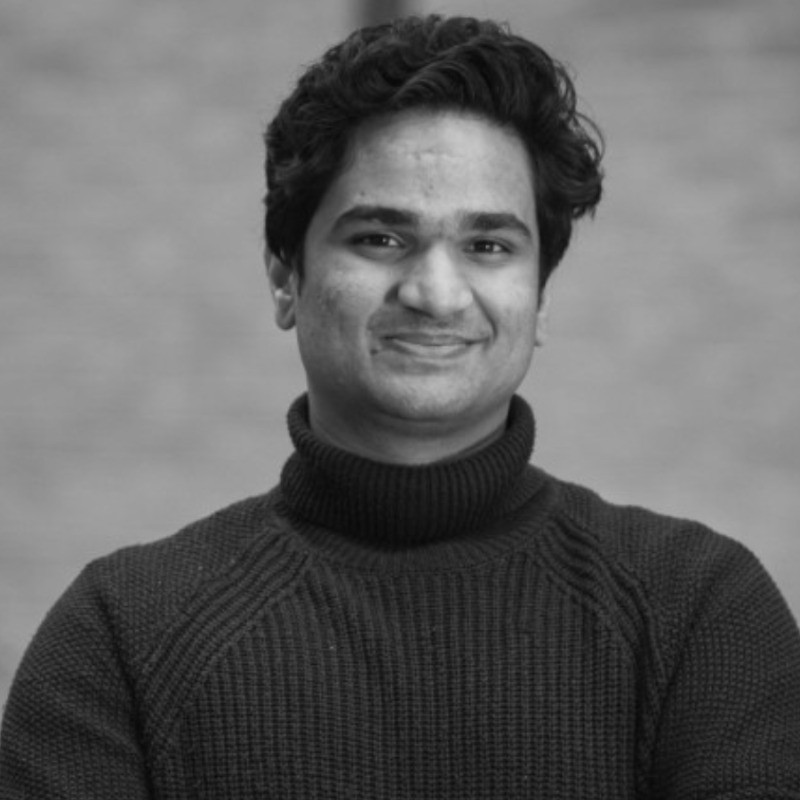
\includegraphics[width=2.3cm,height=2.3cm,keepaspectratio]{photo.jpg}
\end{minipage}

\section{Career Summary}
\begin{itemize}
\item Automation Test \& Validation Engineer with dual degrees in Mechanical Engineering and Management Engineering (Politecnico di Milano).
\item Solid foundation in automated machinery verification, PLC control logic testing (Siemens TIA Portal, Allen-Bradley/Rockwell), and commissioning within regulated environments.
\item Experienced in test protocol execution (FAT/SAT, IQ/OQ), sensor signal verification (pressure, temperature, flow, voltage), and P\&ID/electrical schematic interpretation.
\item Proven track record in automated diagnostic scripting, system troubleshooting, and cross-functional collaboration with quality assurance and engineering teams.
\end{itemize}

\section{Technical Skills}
\begin{itemize}
\item \textbf{Industrial Automation \& PLC} -- Siemens TIA Portal (S7-1200/1500), Allen-Bradley (RSLogix 5000), Rockwell, Automation Studio, HMI/SCADA Interfaces
\item \textbf{Validation \& Compliance} -- Test Protocol Execution, FAT/SAT, IQ/OQ Documentation, GMP Alignment, P\&ID \& Electrical Schematic Reading
\item \textbf{Instrumentation \& Diagnostics} -- Sensor Verification, Temperature/Pressure Transmitters, Signal Calibration (4-20mA, 0-10V), Multimeter, Oscilloscope
\item \textbf{Scripting \& Systems} -- Python, C++, Bash, Linux, SQL, Automated Test Frameworks, Git, Root Cause Analysis
\item \textbf{Protocols \& Networks} -- Industrial Ethernet, Profinet, Modbus, OPC UA, REST APIs
\end{itemize}

\section{Visa \& Language}
\begin{itemize}
\item \textbf{Language} -- Italian (Conversational / Intermediate), English (Fluent / Professional), Hindi (Native)
\item \textbf{Work Authorization} -- European Long Term Residence Permit (No Visa Sponsorship required). Driving License (Patente B). Available for on-site travel.
\end{itemize}

\section{Professional Experience}
\role{\href{https://flowspace.co}{FlowSpace.co}}{Automation Test \& Systems Lead}{London, UK / Remote}{Mar 2024 -- Ongoing}
\begin{itemize}
\item \textbf{Automated Testing \& Systems Validation:}
\begin{itemize}[label=--]
\item Architected automated verification suites and continuous test harnesses for distributed process control pipelines and IoT gateways.
\item Executed structured test protocols evaluating system telemetry, signal response times, and failure-mode recovery under simulated operating loads.
\item Authored technical qualification documents, acceptance criteria reports, and debugging procedures for field commissioning engineers.
\end{itemize}
\item \textbf{Quality Assurance \& Continuous Improvement:}
\begin{itemize}[label=--]
\item Managed regression test runs and diagnostic logging, detecting and isolating synchronization anomalies across interconnected platforms.
\item Collaborated closely with cross-border development and quality teams to implement root-cause corrective actions, ensuring 99.9\% uptime.
\end{itemize}
\item \textit{Tools: Python, Linux, Bash, Automated Test Frameworks, REST APIs, Git, Jira}
\end{itemize}

\role{Urlink}{Systems Automation Engineer}{Milan, Italy}{Jul 2023 -- Feb 2024}
\begin{itemize}
\item Conducted functional testing, sensor calibration, and signal integrity checks on industrial automation machinery prior to factory delivery (collaudo).
\item Verified PLC I/O configurations, safety interlocks, and communication modules following engineering schematics and functional specifications.
\item Formulated detailed test matrices and commissioning checklists covering mechanical, electrical, and control logic sub-assemblies.
\end{itemize}

\role{UltraStrategy}{Automation Developer}{Remote, Germany}{Sep 2022 -- Jun 2023}
\begin{itemize}
\item Built automated data collection scripts monitoring industrial machinery performance and operational throughput metrics across production sites.
\item Automated routine test data extraction, transforming multi-channel sensor logs into structured compliance validation reports.
\end{itemize}

\section{Education}
\role{Politecnico di Milano}{M.Sc. in Management Engineering (Digital Business \& ICT)}{Milan, Italy}{2020 -- 2023}
\role{Thapar Institute of Engineering and Technology}{B.E. in Mechanical Engineering}{Punjab, India}{2014 -- 2018}

\end{document}
